\documentclass{"../../res/univ-projet"}
\usepackage[utf8]{inputenc}
\usepackage[T1]{fontenc}
\usepackage[francais]{babel}
\usepackage{colortbl}
\usepackage{algorithm}
\usepackage{algorithmic}
\usepackage{listings}


\logo{../../res/logo_univ.png}
\title{Architecture Logicielle}
\author{Damien \bsc{Picard}}
\projet{M1SSI}
\projdesc{Projet de génération d'OTP}
\filiere{M1SSI}
\version{2.1a}
\relecteur{Adrien \bsc{Smondack}}
\signataire{\bsc{Bardet} Magali}
\date{Avril 2014}

\histentry{2.1a}{04/04/2014}{Version PAM}
\histentry{2.0}{18/02/2014}{Version post état de l'art}
\histentry{1.2}{16/01/2014}{Version pour la revue de lancement}
\histentry{1.1}{15/12/2013}{Ajout des modifications demandées par le client}
\histentry{1.0}{01/12/2013}{Version relue et corrigée}
\histentry{0.1}{21/11/2013}{Premier jet}

% -----------------------------------------------------------------------------
\lstset{ %
  backgroundcolor=\color{white},   % choose the background color; you must add \usepackage{color} or \usepackage{xcolor}
  basicstyle=\footnotesize,        % the size of the fonts that are used for the code
  breakatwhitespace=false,         % sets if automatic breaks should only happen at whitespace
  breaklines=true,                 % sets automatic line breaking
  captionpos=b,                    % sets the caption-position to bottom
  commentstyle=\color{green},    % comment style
  deletekeywords={...},            % if you want to delete keywords from the given language
  escapeinside={\%*}{*)},          % if you want to add LaTeX within your code
  extendedchars=true,              % lets you use non-ASCII characters; for 8-bits encodings only, does not work with UTF-8
  keepspaces=true,                 % keeps spaces in text, useful for keeping indentation of code (possibly needs columns=flexible)
  keywordstyle=\color{blue},       % keyword style
  language=C,                      % the language of the code
  morekeywords={*,secret,uint64_t},         % if you want to add more keywords to the set
  numbers=left,                    % where to put the line-numbers; possible values are (none, left, right)
  numbersep=5pt,                   % how far the line-numbers are from the code
  numberstyle=\tiny\color{gray},   % the style that is used for the line-numbers
  rulecolor=\color{black},         % if not set, the frame-color may be changed on line-breaks within not-black text (e.g. comments (green here))
  showspaces=false,                % show spaces everywhere adding particular underscores; it overrides 'showstringspaces'
  showstringspaces=false,          % underline spaces within strings only
  showtabs=false,                  % show tabs within strings adding particular underscores
  stepnumber=1,                    % the step between two line-numbers. If it's 1, each line will be numbered
  stringstyle=\color{mauve},       % string literal style
  tabsize=2,                       % sets default tabsize to 2 spaces
  title=\lstname                   % show the filename of files included with \lstinputlisting; also try caption instead of title
}

%------------------------------------------------------------------------------

\begin{document}
\maketitle
%-------------------------------------------------------------------------------
\section{Objet}
Ce document a pour but de préciser les détails techniques du module PAM gérant une authentification
par mot de passe jetable.

\section{Documents de référence}
\subsection{Documents de spécifications}
\begin{tabular}{p{1,5cm}>{\raggedright\arraybackslash}p{13cm}}
{[ANS10]} & {ANSSI. Référentiel général de sécurité. \href{http://www.ssi.gouv.fr/fr/reglementation-ssi/referentiel-general-de-securite}{http://www.ssi.gouv.fr/fr/reglementation-ssi/referentiel-general-de-securite}, 2010.}
\tabularnewline
\\
{[MvOV97]} & {Alfred J. Menezes, Paul C. van Oorschot, and Scott A. Vanstone. Handbook of applied cryptography. CRC Press Series on Discrete Mathematics and its Applications. CRC Press, Boca Raton, FL, 1997. With a foreword by Ronald L.Rivest.}
\tabularnewline
\\
{[RFC98]} & {A One-Time Password System. \href{http://tools.ietf.org/html/rfc2289}{http://tools.ietf.org/html/rfc2289}, 1998.}
\tabularnewline
\\
{[RFC05]} & {HOTP:An HMAC-Based One-Time Password Algorithm \href{http://tools.ietf.org/html/rfc4226}{http://tools.ietf.org/html/rfc4226}, 2005.}
\tabularnewline
\\
{[RFC06]} & {Generic Message Exchange Authentication for the Securer Shell Protocol (SSH).\href{http://tools.ietf.org/html/rfc4256}{http://tools.ietf.org/html/rfc4256}, 2006.}
\tabularnewline
\\
{[RFC07]} & {The EAP Protected One-Time Password Protocol (EAP-POTP). \href{http://tools.ietf.org/html/rfc4793}{http://tools.ietf.org/html/rfc4793}, 2007.}
\tabularnewline
\\
{[RFC11]} & {HOTP: Time-Based One-Time Password Algorithm \href{http://tools.ietf.org/html/rfc6238}{http://tools.ietf.org/html/rfc6238}, 2011.}
\tabularnewline
\\
{[goo]} & {Google Authenticator \href{https://code.google.com/p/google-authenticator/}{https://code.google.com/p/google-authenticator/}.}
\tabularnewline
\\
\end{tabular}

%-------------------------------------------------------------------------------
\section{Configuration requise}

\subsection{Périphériques et matériel spécifiques}
\begin{tabular}{|c|p{0.3\textwidth}|p{0.4\textwidth}|}
\hline
\rowcolor{gray}
\textcolor{white}{\bfseries Identifiant} & 
\textcolor{white}{\bfseries Description} &
\textcolor{white}{\bfseries Justification} \\
\hline
PR-M\_001 &
Machine capable d'exécuter un système d'exploitation GNU/Linux. & 
Le module PAM réalisé n'est prévu pour fonctionner que sur un système GNU/Linux. \\
\hline
\end{tabular}

\subsection{Système d'exploitation}
\begin{tabular}{|c|p{0.3\textwidth}|p{0.4\textwidth}|}
\hline
\rowcolor{gray}
\textcolor{white}{\bfseries Identifiant} & 
\textcolor{white}{\bfseries Description} &
\textcolor{white}{\bfseries Justification} \\
\hline
OS\_001& 
GNU/Linux kernel 3.x / glibc >= 2.15, présence de /dev/random et /dev/urandom 
pour un module PAM &
Le but du projet est de développer un module PAM pour pouvoir s'authentifier
à l'aide de mot de passe jetable. PAM est une technologie qui n'est disponible
que sur certains systèmes de type UNIX.\\
\hline
\end{tabular}

\subsection{Pré-requis logiciels}
\begin{tabular}{|c|p{0.3\textwidth}|p{0.4\textwidth}|}
\hline
\rowcolor{gray}
\textcolor{white}{\bfseries Identifiant} & 
\textcolor{white}{\bfseries Description} &
\textcolor{white}{\bfseries Justification} \\
\hline
PR-L\_001 &
Bibliothèque PAM > 1.0 &
Le développement d'un module PAM suppose la présence des bibliothèques permettant
le fonctionnement de PAM sur le système. \\
\hline
PR-L\_002 &
Bibliothèque OpenSSL avec SHA1 &
Les algorithmes retenus sont basés sur la fonction de hachage SHA1. Pourra être réimplémenté. \\
\hline
PR-L\_003 &
Bibliothèque math &
Cette bibliothèque est utilisée pour la fonction d'exponentiation. \\
\hline
PR-L\_004 &
Bibliothèques de test unitaire C Check &
Nécessaire pour la compilation des tests réalisés avec ce framework.\\
\hline
PR-L\_005 &
Système de gestion de configuration \verb?cmake? > 2.8.5&
Nécessaire pour la construction du projet\\
\hline
PR-L\_006 &
Système de gestion de construction \verb?make? &
Nécessaire pour la compilation du projet\\
\hline
PR-L\_007 &
Compilateur \verb?gcc? > 4.0 &
Nécessaire pour compiler le projet\\
\hline
\end{tabular}


%-------------------------------------------------------------------------------
\part*{Architectures statiques}
\section{Structure générale du système}
% TODO: refaire ce graphique.
%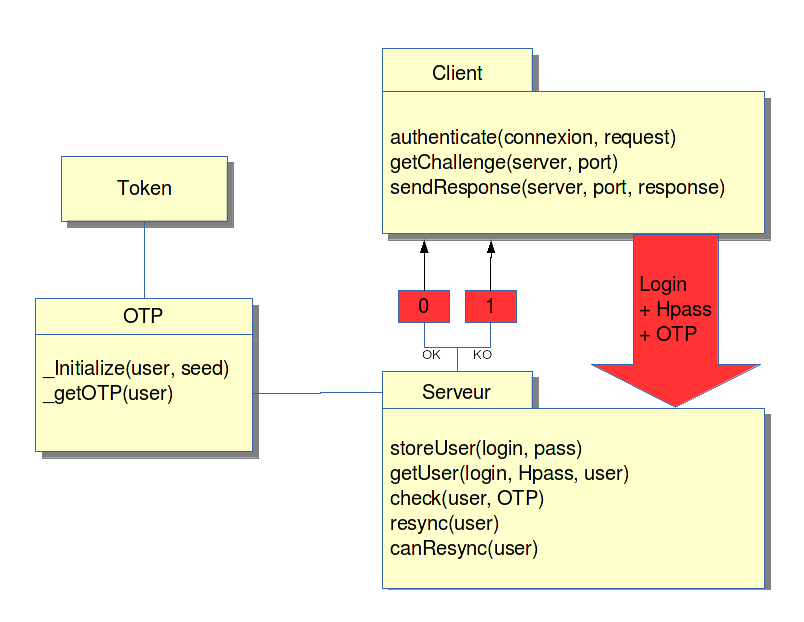
\includegraphics[width=\textwidth]{../graphics/architecture.png}

%------------------------------------------------------------------------------
\subsection{Gestion des secrets}
\subsubsection{Rôle}
Avant de générer un mot de passe jetable il faut que les applications se mettent
d'accord sur un secret. Pour une implémentation en C, avoir une structure de données
plus évoluée qu'un simple buffer permet de s'épargner une gestion fastidieuse des secrets.

\subsubsection{Services offert}
Ce module fournit une structure de données appelée \verb?secret? qui permet de représenter
un secret en mémoire.

Ce module fourni des fonctions de création de secret.
\begin{lstlisting}
secret createSecret(int length);
secret createRandomSecret(int length);
secret hexToSecret(char * buffer);
secret textToSecret(char * buffer);
\end{lstlisting}
Ainsi que deux fonctions pour obtenir des représentations différentes du secret.
\begin{lstlisting}
char * getHexRepresentation(secret key, char * buffer, int length);
char * getTextRepresentation(secret key, char * buffer, int length);
\end{lstlisting}
Une fonction pour obtenir des informations relatives au secret.
\begin{lstlisting}
int getLength(secret key);
\end{lstlisting}
Une fonction pour libérer les ressources associées au secret en machine.
\begin{lstlisting}
int destroySecret(secret key);
\end{lstlisting}

\subsubsection{Procédé de développement}
On commencera par définir la structure de données, comment on représente le secret dans la mémoire
puis on développera toutes les fonctions en conséquences.

\subsubsection{Taille et complexité}
Cette fonction consiste majoritairement en de la manipulation de buffer et de la conversion d'un
format de données en un autre. L'équipe étant supposée habituée à ces tâches le développement devrait être 
rapide.

\subsection{Générateur d'OTP}
Les implémentations retenues après études des RFC sont TOTP et HOTP. TOTP
n'étant qu'une variante d'HOTP seul un générateur d'HOTP sera programmé.
on fera varier ses paramètres afin d'obtenir un générateur de TOTP.

\subsubsection{Rôle}
Le rôle de cette partie du projet est de générer des mots de passes jetables
à partir d'un secret, d'un compteur et une longueur. 

Pour générer des mots de passes selon le protocole TOTP on passera le temps UTC
divisé par une période en tant que compteur.

\subsubsection{Services offerts}
Ce module fournit la fonction:
\begin{lstlisting}
int generate_otp(secret s, uint64_t counter, int len);
\end{lstlisting}


\subsubsection{Procédé de développement}
On commencera par implémenter les fonctions utilitaires qui ne seront pas accessibles en
dehors du module. Ensuite nous implémenterons la génération d'OTP.

\subsubsection{Taille et complexité}
C'est l'une des parties nouvelles et cruciale du projet. Non seulement car il n'y 
a que peu de moyen de vérifier que le générateur d'OTP fonctionne réellement. Et
qu'il faut en plus être compatible avec les RFC HOTP et TOTP.

De plus un certain nombre de modifications peuvent être apportées a posteriori comme 
l'indépendance vis a vis des bibliothèques OpenSSL et libmath.

\subsection{Le module PAM}
\subsubsection{Rôle}
Le but de ce composant est de fournir un module pour PAM et permettre de s'authentifier
à l'aide de mots de passe jetables.

\subsubsection{Services offerts}
Ce module permettra d'intégrer une authentification par OTP dans un service utilisant PAM
en insérant la ligne:
\begin{verbatim}
auth required pam_otp.so
\end{verbatim}
Il sera aussi possible de gérer la mise à jour du secret en insérant la ligne:
\begin{verbatim}
password required pam_otp.so
\end{verbatim}


\subsubsection{Procédé de développement}
On commencera par fournir la fonction minimale du module, c'est à dire l'authentification. Viendra
ensuite la mise à jour de secret puis la gestion des éventuelles options.

\subsubsection{Taille et complexité}
C'est la deuxième partie cruciale et nouvelle du projet, il faut d'abord que l'équipe s'approprie
la technologie ensuite il suffira de développer les quelques fonctions que le module doit fournir.

%-------------------------------------------------------------------------------
\subsection{Justification des choix techniques}
On utilisera le langage C pour développer le module C qui est le langage recommandé par
les développeurs de PAM. On utilisera aussi la bibliothèque OpenSSL pour SHA1 et la libmath
pour la fonction puissance. Ces deux bibliothèques pourront ensuite être remplacées par une implémentation
de ces deux fonction propre à notre projet.

%---------------------------------------------------------------------------------        
\part*{Architecture dynamique}
\section{Demande de secret}
La demande de secret sera permise grâce a l'implémentation des fonctions requises au sein du
module. Par exemple une fois l'application configurée pour déléguer la gestion de secret au
module l'application pourra faire appel à ces fonctions.
\newline
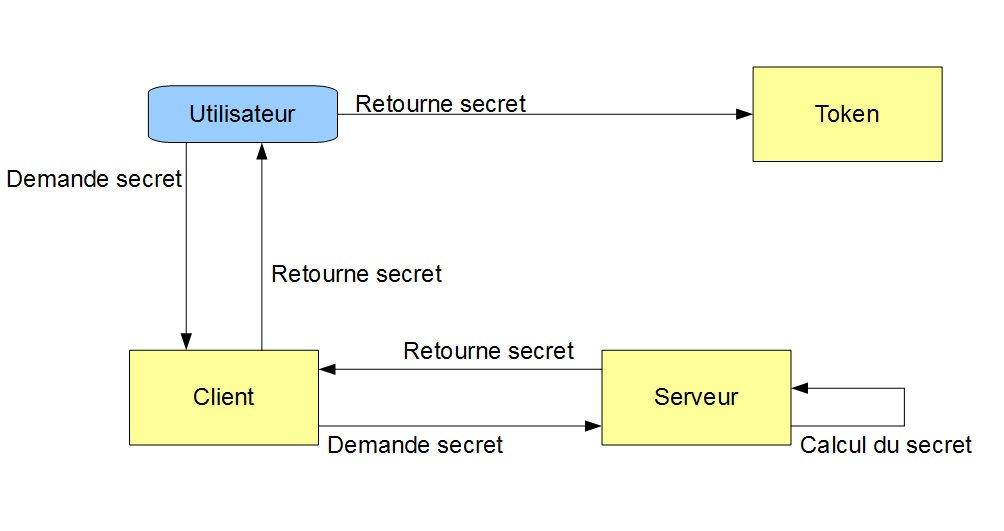
\includegraphics[width=\textwidth]{../graphics/association.jpg}

\section{Authentification}
L'authentification sera fournie par le module PAM. Une application qui fait appel à PAM pour gérer
les authentifications pourra donc être configurée pour utiliser des mots de passe jetables.

Typiquement lors d'une connexion en SSH si le serveur est configuré pour utiliser PAM et que le module
d'authentification par OTP est dans la liste pour gérer l'authentification alors un OTP sera demandé
à l'utilisateur. Le module PAM décidera de la validité du mot de passe.
\newline
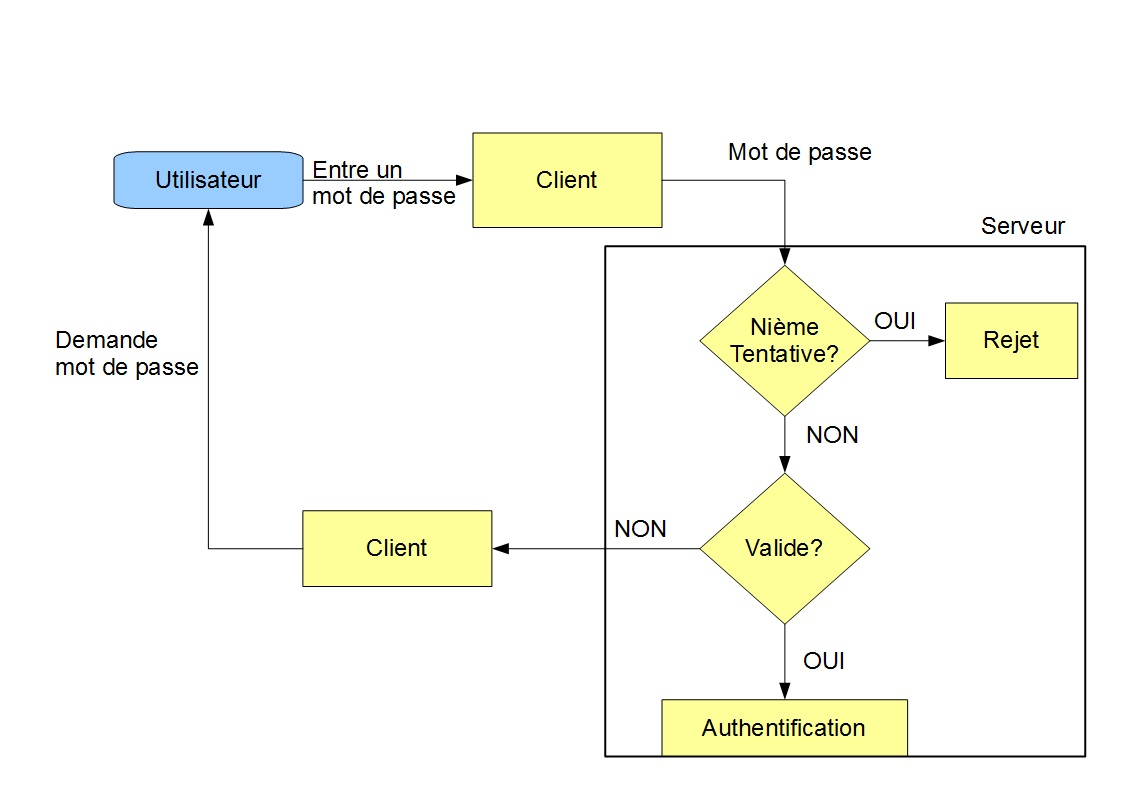
\includegraphics[width=\textwidth]{../graphics/authentification.jpg}
\end{document}
